%
% Unless otherwise indicated, the copyright in this material is 
% owned by Joerg Evermann. This material is licensed to you under the 
% Creative Commons by-attribution non-commercial license (CC BY-NC 4.0)}
%
\section*{Learning Goals}

After reading this chapter, you should be able to:
\begin{itemize}
   \item Understand property graphs and the concept of nodes and edges.
   \item Understand when graph databases are preferrable over relational databases.
   \item Define basic graphs using Cypher.
   \item Create graph structures appropriate for different types of queries. 
   \item Translate a relational database schema into a graph database definition.
   \item Retrieve information from a graph database using Cypher, including filtering and aggregation of information.
\end{itemize}

\section{Introduction}

Graph databases are one type of \emph{NoSQL} databases, an acronym for ''Not Only SQL''. NoSQL databases emerged as a response to the limitations of traditional relational database systems and the evolving needs of modern applications. The concept and the term ''NoSQL'' gained prominence in the late 2000s, but its roots can be traced back to earlier innovations in database technology.

The rise of the internet and web applications in the 1990s and 2000s led to unprecedented amounts of data and new types of data that did not fit neatly into the rows and columns of relational databases. Companies like Google and Amazon faced challenges in scaling their databases to meet the demands of huge amounts of web traffic and large, unstructured data sets. This led to the development of new database systems like Google's Bigtable and Amazon's Dynamo, which laid the groundwork for NoSQL databases.

NoSQL\index{NoSQL database} databases were designed to overcome the scalability, performance, and flexibility limitations of traditional relational databases. Unlike relational databases that use a fixed table structure, NoSQL databases utilize a variety of data models, including key-value, document, and graph formats. This diversity allows them to handle a wide array of data types and structures efficiently.

Key benefits of NoSQL databases include their ability to scale horizontally across many servers, offering significant advantages in handling large-scale, high-volume applications and big data. They also deliver high performance, particularly with large volumes of data and concurrent read/write operations, due in part to their typical emphasis on eventual data consistency over strict ACID compliance (atomicity, consistency, isolation, and durability of database transactions).

The schema-less nature of NoSQL databases provides more agility in application development. Developers can iterate quickly without needing to restructure databases every time the application evolves. This flexibility is especially valuable in agile software development environments and for applications dealing with diverse, unstructured, or rapidly evolving data sets.

Moreover, many NoSQL databases natively support modern data formats like JSON, aligning well with current web and mobile applications. This can simplify the development process, as the same data format can be used throughout the application stack.

However, the strenghts of NoSQL databases also bring some drawbacks. The lack of a fixed schema means that data integrity cannot be ensured using typing of columns, primary keys on unique identifiers, or referential integrity with foreign keys. NoSQL databases also do not typically make correctness guarantees for concurrent transactions that come from the ACID properties of relational databases. Instead, they guarantee that eventually the data will be consistent, but applications and users may occasionally see inconsistent data. Generally NoSQL databases are less suitable for high-volume concurrent update transaction processing; these application types are better supported by relational databases. Instead, NoSQL databases are better suited for applications that may require complex queries but relatively infrequent updates, few concurrent update transactions, and updates of single data elements at a time.

Graph databases\index{Graph database} are designed to store and query relationships in data. They represent data as nodes, akin to entities in a relational database, and relationships between these nodes. This structure is particularly suited for handling complex, interconnected data and is highly efficient in scenarios where relationships are as important as the data itself. Graph databases gained significant traction driven by the increasing complexity of data and the limitations of relational databases in efficiently handling highly connected or networked data. The proliferation of social networks, recommendation systems, and other applications dealing with complex relationships between data entities spurred the development of graph databases.

Unlike relational databases that require computationally intensive join operations to establish connections between data in different tables, graph databases are designed to store relationships as first-class objects. This means that queries on interconnected data are faster and more efficient, as they exploit the direct connections between nodes. Additionally, graph databases are schema-less or have flexible schemas, allowing for more agility in adapting to changing data requirements.

\section{Use Cases}

Graph databases have become increasingly important in various industries due to their ability to efficiently model and query complex relationships and interconnected data that arise in those applications. 

In \emph{fraud detection}, graph databases are used to uncover patterns that are indicative of fraudulent activities. They can map complex transaction networks and identify unusual patterns, such as circular transactions or abnormally close relationships between entities, that might signal fraud. The ability to quickly traverse and analyze complex networks of data helps in real-time detection and prevention of fraud.

For \emph{IT infrastructure monitoring}, graph databases offer a way to model complex networks of servers, devices, and applications. They can track the relationships and dependencies between various components of an IT system. This is invaluable for root cause analysis, where understanding the impact of an issue in one part of the system on the rest is crucial for quick resolution.

Graph databases power \emph{recommender engines} by capturing and analyzing relationships between users, their preferences, and products. They can efficiently traverse these relationships to generate personalized recommendations based on a user's past behavior and the behavior of similar users.

In \emph{social media}, graph databases are used to model the complex relationships between users, their friends, and their activities. They help in understanding social dynamics, optimizing content delivery, and enhancing user engagement by providing insights into how users are connected and how information flows through these networks.

For \emph{supply chain management}, graph databases can model the entire supply chain network, including suppliers, production facilities, distribution centers, and retail outlets. This aids in optimizing routes, managing inventories, and identifying vulnerabilities in the supply chain, such as single points of failure.

In the \emph{financial sector}, graph databases are utilized for risk assessment, compliance, customer service, and understanding client relationships. They help in mapping and analyzing complex networks of transactions and customer relationships, which is critical for identifying risks, ensuring compliance with regulations, and offering personalized financial services.

In \emph{life sciences}, graph databases play a significant role in drug discovery, genomics, and protein analysis. They are used to model complex biological systems and relationships, such as gene interactions, protein pathways, and patient data, assisting in research and the development of personalized medicine.

In each of these domains, the key advantage of graph databases lies in their ability to naturally represent complex networks and relationships. This allows for more intuitive data modeling, faster querying, and the extraction of insights that would be difficult or impossible to obtain with traditional relational databases.

\section{Graph Database Languages}

In contrast to the standardized SQL language for relational databases, graph databases use various query languages designed to leverage their unique structure and efficiently handle complex queries that involve interconnected data. One of the more prominent ones is the Cypher language\index{Cypher (query language)}, introduced and primarily used in the Neo4j graph database system since 2011 but opened for use in other systems in 2015 as the openCypher project. It is a declarative language\footnote{A declarative query language allows the user to specify \emph{what} data to retrieve. In contrast, an imperative/procedural query language requires the user to specify \emph{how} to retrieve data.}, known for its expressive and readable syntax tailored for describing patterns in graphs. Cypher allows for easy querying of nodes, relationships, and paths and includes powerful features for filtering, pattern matching, and aggregating data.

Another notable query language is Gremlin\index{Gremlin (query language)}, part of the Apache TinkerPop graph computing framework. Development began in 2009 and is ongoing. Gremlin is versatile and functional, allowing for imperative and declarative querying across different graph databases. It is known for its flexibility and ability to execute both simple and complex traversals, making it suitable for a wide range of applications.

SPARQL\index{SPARQL protocol and RDF query language} (a recursive acronym for ''SPARQL Protocol and RDF Query Language'') is a query language used primarily for querying RDF (Resource Description Framework) data, often found in semantic web applications. Its development is overseen and standardized by the W3C (World Wide Web Consortium), beginning in 2008 with a major update in 2013. It is particularly suited to querying and manipulating data stored in RDF format, and is widely used in applications that require linking diverse data sources, such as knowledge graphs.

Additionally, some graph databases support SQL-like query languages with extensions to handle graph-specific structures. These languages make it easier for users familiar with SQL to transition to graph databases. An example is GraphQL, developed by Facebook in 2015. 

The lack of a standard query language in the graph database realm has led to fragmentation. This fragmentation can pose challenges for users and developers, such as a steeper learning curve and difficulty in transitioning between different graph database systems. In response, the forthcoming standardized GQL\index{Graph query language}\index{GQL|see{Graph query language}} (Graph Query Language) is a new graph query language specifically designed for interacting with graph databases. The development of GQL is overseen by ISO/IEC JTC 1, the same joint technical committee responsible for the SQL standard. Its design is expected to draw on the strengths of existing languages, offering robust features for graph traversal, pattern matching, and manipulation of graph structures while maintaining readability and ease of use. A first version of the GQL standard was expected for 2023.

\section{The Neo4j Graph Database Management System}

Cypher is the query language for Neo4j, one of the most popular graph database systems. It was specifically designed for querying the graph data in Neo4j, making it easy to work with complex graph structures. Cypher's syntax is intuitive and expressive, focusing on the clarity of graph patterns and drawing inspiration from SQL and other declarative query languages. Its pattern matching approach was styled after the SPARQL language. Key characteristics and features of Cypher include:

\begin{itemize}
\item \emph{Graph Pattern Matching}: Cypher provides the ability to expressively describe graph patterns. It uses a syntax where nodes and relationships in the graph are depicted using parentheses (representing nodes) and arrows (representing relationships). This makes it visually intuitive to understand the queries and the graph patterns they represent.

\item \emph{Rich Filtering Capabilities}: Cypher includes robust filtering capabilities, enabling users to write queries that can filter nodes and relationships based on various criteria, including properties and patterns.

\item \emph{Aggregation and Sorting}: Like SQL, Cypher allows for aggregating data, performing calculations, and sorting results. It provides functions for counting, summing, averaging, and other common aggregations.

\item \emph{Pathfinding and Graph Algorithms}: Cypher can handle common graph queries such as shortest path, reachable nodes, and more.

\item \emph{Subqueries and Joins}: Cypher supports subqueries and various forms of joins, enabling complex queries that can span multiple parts of the graph.

\item \emph{Extensibility}: Cypher can be extended with user-defined procedures and functions, allowing for custom logic and advanced processing capabilities.
\end{itemize}

Similar to SQL queryies, Cypher queries have multiple clauses, specifying a ''query pipeline'' for selecting, filtering, and sorting data. Unlike SQL, Cypher queries allow graph reading and graph updating in the same Cypher statement. 

Neo4j offers a number of options for running the Neo4j database management system, among them a limited developer version called ''Neo4j desktop'' and a free, open-source community edition that is usually accessed through a web interface (''Neo4j browser''). Table~\ref{tab:neo4jinfo} provides links to useful documentation of the Neo4j database and the Cypher language.

\begin{tcolorbox}[colback=alert]
The community edition is installed in the course virtual machine and enabled to run when the machine is started. You can access Neo4j Browser (Figure~\ref{fig:neo4jbrowser}) at \url{http://localhost:7474} with the username ''\textbf{neo4j}'' and the password ''\textbf{busi4720}''. 
\end{tcolorbox}

\begin{table}
\renewcommand{\arraystretch}{1.5}
\centering
\small
\begin{tabular}{l|l} \hline
Getting Started & \url{https://neo4j.com/docs/getting-started/} \\ 
Cypher Manual & \url{https://neo4j.com/docs/cypher-manual} \\
Graph Data Science & \url{https://neo4j.com/docs/graph-data-science} \\ 
APOC Library & \url{https://neo4j.com/docs/apoc/current/} \\ 
Use Cases & \url{https://neo4j.com/use-cases/} \\
Resources & \url{https://neo4j.com/resources/} \\
\hline
\end{tabular}
\caption{Neo4j Documentation}
\label{tab:neo4jinfo}
\end{table}

\begin{figure}
\centering
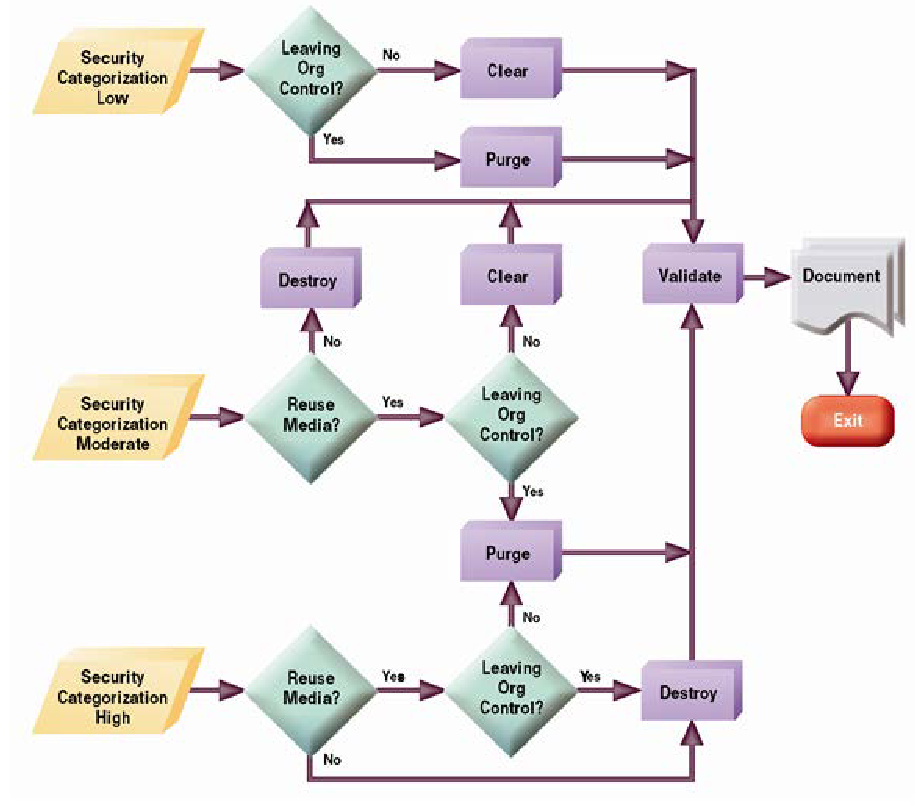
\includegraphics[width=.75\textwidth]{screen1.png}
\caption{Neo4j Browser interface}
\label{fig:neo4jbrowser}
\end{figure}

\section{Introduction to Cypher}

\paragraph*{Nodes}
Figure~\ref{fig:sample-cypher} shows how nodes and relationships are represented in the Cypher syntax. In Neo4j, nodes\index{Node (in Neo4j)} may be labelled with zero, one, or more labels. Labels\index{Label (in Neo4j)} are not types; a label does not specify anything about the information associated with a node, it merely serves to categorize or classify nodes. Nodes may have properties\index{Property (in Neo4j)}, specified as key--value pairs in JSON syntax. Graph nodes are written with normal round parentheses, with the set of their properties in curly brackets. Both the variable name for the node and the node labels are optional.

\begin{cyphercode}
(variable : Label1:Label2:Label3 ... {k1:v1, k2:v2, k3:v3 ....})
\end{cyphercode}


\begin{figure}
\centering
\includegraphics[width=.75\textwidth]{sample-cypher.png}
\scriptsize{\url{https://neo4j.com/docs/getting-started/_images/sample-cypher.svg}}
\caption{Sample Cypher syntax}
\label{fig:sample-cypher}
\end{figure}

\paragraph*{Relationships} Relationships\index{Relationship (in Neo4j)} are directed connections between two nodes. Unlike nodes, relationships only have a single label. But like nodes, they can have properties specified as key--value pairs in JSON syntax. Relationships are written as ''lines'' between nodes, directed or undirected, with an optional variable name and relationship label in square brackets. 

\begin{samepage}
\begin{cyphercode}
// Undirected, used in pattern
()-[variable : Label]-()  
// Directed 
()-[variable : Label]->() 
// Directed
()<-[variable : Label]-() 
// Unlabelled, no variable
()-[]-()    
()-->()
()<--()
\end{cyphercode}
\end{samepage}

\begin{tcolorbox}[colback=alert]
\emph{Only directed relationships can be created in a Neo4j graph, but undirected relationships can be used in a pattern to query a graph}. \\

Directionality of relationships is important and matters for querying a graph. A directed relationship \texttt{-->} will match a directed pattern \texttt{-->} or an undirected pattern \texttt{--} but not \texttt{<--}. 
\end{tcolorbox}

\paragraph*{Path}
A path\index{Path (in Neo4j)} in Neo4j is a sequence of alternating nodes and relationships, beginning and ending with a node.

\paragraph*{Patterns and Querying}

Graph patterns\index{Pattern (in Cypher)} are used with the MATCH query keyword and describe either a node or a path that is to be searched for in the graph. When an instance of a pattern is found, any variable names in the pattern are bound to the corresponding nodes and relationship in the graph and the bound pattern is returned in the result set.

For example, consider the following simple pattern matching query. The \texttt{MATCH} clause specifies the pattern to match. The pattern here is a node, indicated by the use of round parentheses, and only a variable name \texttt{n} is specified, no labels or property values. This means that this pattern matches all nodes in the graph database and returns them in the variable names \texttt{n}.

\begin{cyphercode}
MATCH (n)
\end{cyphercode}

The next pattern matching query adds a label \texttt{Person} to the node specification. This means the pattern matches only those nodes that are labelled as Person and returns them in the variable named \texttt{p}.

\begin{cyphercode}
MATCH (p:Person)
\end{cyphercode}

Patterns can include property values to match. The following pattern matches all Person nodes that contain an attribute \texttt{name} with value 'Joe' and returns them in the variable \texttt{p}.

\begin{cyphercode}
MATCH (p:Person {name: 'Joe'})
\end{cyphercode}


\section{Defining Graphs in Cypher}

Nodes or relationships in a graph can be created using the MERGE or CREATE statements in Cypher. As the name indicates, CREATE will create a node or relationship. In contrast, MERGE will check whether the node or relationship exists and only create it when it does not yet exist in the graph. Consider the example graph shown in Figure~\ref{fig:johnsallyexample}. The following Cypher codes creates this graph:

\begin{figure}[h]
\centering
\includegraphics[width=.75\textwidth]{screen4.png} \\

\scriptsize{\url{https://neo4j.com/docs/getting-started/_images/modeling_johnsally_properties-arr.svg}}
\caption{Example graph}
\label{fig:johnsallyexample}
\end{figure}

\begin{samepage}
\begin{cyphercode}
// Create nodes
MERGE (j:Person {name: "John"})
  ON CREATE SET j.age = 27
MERGE (s:Person {name: "Sally"})
  ON CREATE SET s.age = 32
MERGE (b:Book {title: "Graph Databases"})
  ON CREATE SET b.authors = ["Jim Webber", "Ian Robinson"]
  
// Create relationships
MERGE (j)-[rel1:IS_FRIENDS_WITH]->(s)
  ON CREATE SET rel1.since = "01/09/2013"
MERGE (j)-[rel2:HAS_READ]->(b)
  ON CREATE SET rel2.on = "02/03/2013", rel2.rated = 5
MERGE (s)-[rel3:HAS_READ]->(b)
  ON CREATE SET rel3.on = "02/09/2013", rel3.rated = 4
\end{cyphercode}
\end{samepage}

Note that the six \texttt{MERGE} statements in the above code block are logically related, so that variable names, for example \texttt{j, b} and \texttt{s}, in one \texttt{MERGE} clause can be used to refer to a new node or relationship in a later \texttt{MERGE} clause. While using variable names in a \texttt{MERGE} clause is not mandatory, it is more efficient than having to later query the graph data for a particular node when creating subsequent relationships. The \texttt{ON CREATE SET} clause in the above statements sets one or more property values (separated by commas) of the newly created nodes and relationships. Note that some properties are lists, such as the \texttt{authors} property, indicated by the square brackets of the JSON notation. 

The following \texttt{MATCH} queries can be used to view all nodes and relationships, irrespective of their labels. The first \texttt{MATCH} clause matches all nodes and returns them, the second \texttt{MATCH} clause matches all relationships between any two nodes and returns the relationships, the final query matches any two nodes that are connected by a relationship and returns the set of triples of first node, second node, and relationship.

\begin{samepage}
\begin{cyphercode}
// Query nodes
MATCH (n) RETURN n    
                
// Query relationships
MATCH ()-[r]-() RETURN r              

// Query both together
MATCH (n1)-[r]-(n2) RETURN n1, r, n2  
\end{cyphercode}
\end{samepage}

\noindent The Neo4j Browser interface allows graph visualization and visual exploration of nodes, relationships, and their properties, as shown in Figure~\ref{fig:neo4jgraphviz}.

\begin{figure}[h]
\centering
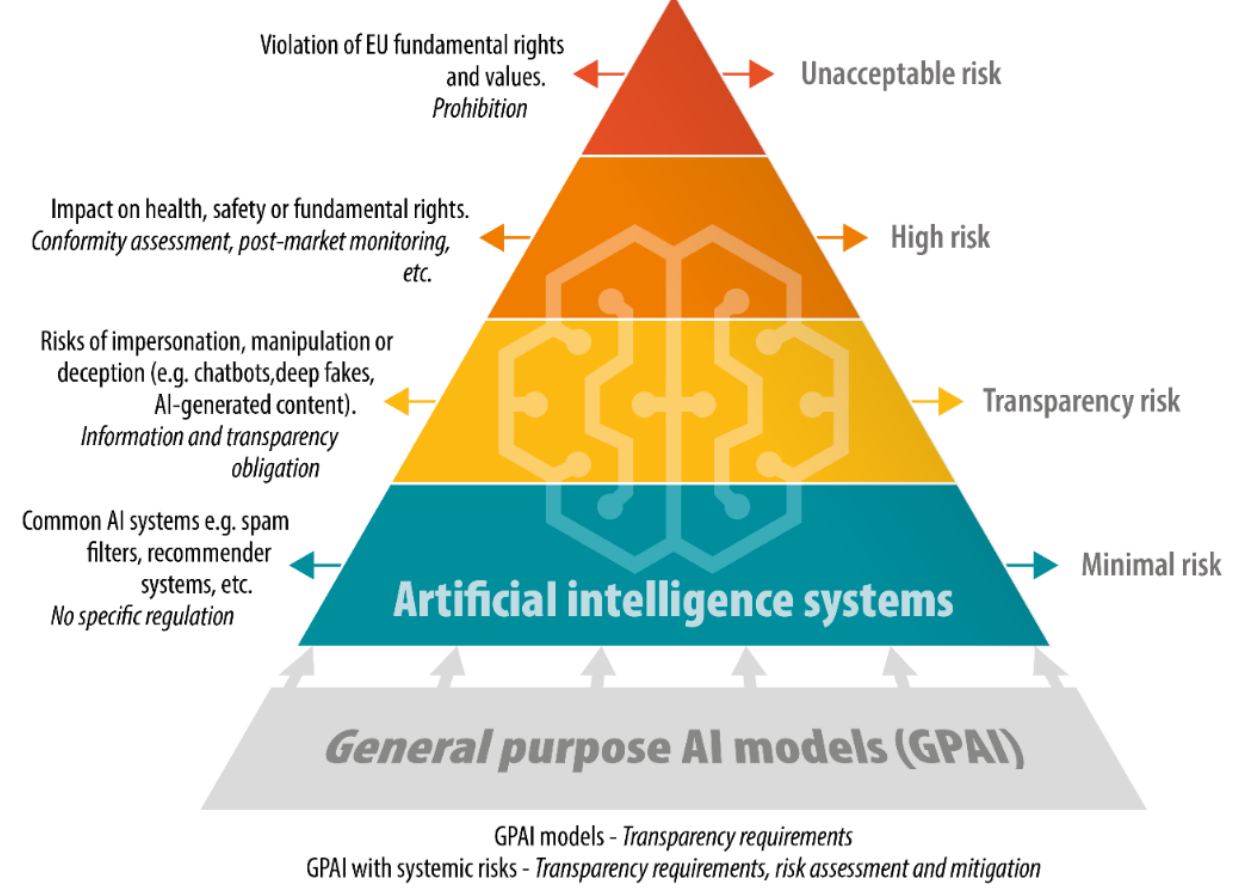
\includegraphics[width=.8\textwidth]{screen2.png}
\caption{Graph Visualization and Exploration in Neo4j Browser}
\label{fig:neo4jgraphviz}
\end{figure}

\begin{tcolorbox}[colback=code]
\subsubsection*{Hands-On Exercise}

Consider the following description:

\begin{quote}
''You are completing the course BUSI 4720 in this semester with a final grade of 100. BUSI 4720 is part of the BCom program where it is offered in the 4th year. BUSI 4720 carries 3 credit hours of academic credit. It is a course on the topic of Business Analytics.''
\end{quote}

Define a graph in Cypher that represents this description:
\begin{enumerate}
  \item Identify nodes, relationships, and properties of nodes and relationships
  \item Use CREATE or MERGE statements to create nodes first, then relationships
  \item Use MATCH to verify your graph is correct.
\end{enumerate}
\end{tcolorbox}

To remove nodes and relationships from a graph, use the \texttt{MATCH} query clause together with a \texttt{DELETE} clause. For example, to clean and remove the Person and Book nodes and relationships between Person and Book nodes created in the previous exercise, use the following Cypher statements:

\begin{cyphercode}
MATCH (:Person|Book)-[r]-(:Person|Book) DELETE r;
MATCH (n:Person|Book) DELETE n;
\end{cyphercode}

To remove \emph{all} relationships and nodes, irrespective of their label, omit node or relationship labels, as in the following Cypher code block. Use with care as this deletes all data in the graph database.

\begin{cyphercode}
MATCH ()-[r]-() DELETE r;
MATCH (n) DELETE n;
\end{cyphercode}

\section{Graph Data Modeling}

When defining a graph, one frequent question is whether to model something as a property of a node or as a relationship to a node. While there is no generally right or wrong answer to this question, the choice of data model depends on the queries to be run against the data, that is, the type of questions that will be asked.

\subsection*{Nodes versus Relationships}

Consider the two graph models in Figures~\ref{fig:propertymodel} and \ref{fig:relationshipmodel}. Both depict the same fact, that there exists a movie with title ''The Matrix'' in two genres, ''Action'', and ''Sci-Fi''. Figure~\ref{fig:propertymodel} models the genres as a property of list type, that contains multiple entries in the list. In contrast, Figure~\ref{fig:relationshipmodel} models the genres as nodes and the fact that the movie is in a genre as a relationship between the movie node and a genre node.

\begin{figure}
\centering
\begin{subfigure}{0.48\textwidth}
    \includegraphics[width=.95\textwidth]{screen5.png}
    \scriptsize{\url{https://neo4j.com/docs/getting-started/\_images/modeling\_genre\_property-arr.svg}}
    \caption{Model as property}
    \label{fig:propertymodel}
\end{subfigure}
\hfill
\begin{subfigure}{0.48\textwidth}
    \includegraphics[width=.95\textwidth]{screen6.png}
    \scriptsize{\url{https://neo4j.com/docs/getting-started/\_images/modeling\_genre\_node-arr.svg}}
    \caption{Model as relationship}
    \label{fig:relationshipmodel}
\end{subfigure}
\hfill
\caption{Equivalent graph models of movie genres}
\label{fig:equivalentmodels}
\end{figure}

The graph model in Figure~\ref{fig:propertymodel} is particularly useful to find the genres for a particular movie, that is, it is useful for queries that focus on the nodes and their properties. However, this model makes it difficult, cumbersome, and inefficient to find movies that share genres. The system has to consider all pairs of movies, and then for each pair of movies iterate through each of their property lists. The following two queries exemplify this. The first query simply filters the Movie nodes for a particular title and returns the genre attribute of the Movie node. 

The second query first identifies all pairs of Movie nodes in the \texttt{MATCH} clause, then uses the \texttt{WHERE} clause to filter those pairs that share entries in their genre attribute. Recall that the genre attributes are lists, so \texttt{x IN m1.genre WHERE x IN m2.genre} checks every element of the second list for every element of the first list. 

\begin{samepage}
\begin{cyphercode}
// find the genres for a particular movie
MATCH (m:Movie {title:"The Matrix"})
RETURN m.genre;

// find which movies share genres
MATCH (m1:Movie), (m2:Movie)
WHERE any(x IN m1.genre 
          WHERE x IN m2.genre)
AND m1 <> m2
RETURN m1, m2;
\end{cyphercode}
\end{samepage}

The graph model in Figure~\ref{fig:relationshipmodel} on the other hand requires a more complex query to find the genres of the movie. However, while more complex, it no less efficient than the corresponding query for the other model above. On the other hand, the query to find movies that share genres becomes easier, more intuitive to write, and more computationally efficient, as the following Cypher queries show.

The first query uses \texttt{MATCH} to first select movies and filter on the movie name, then for that movie \texttt{m} it traverses the \texttt{IN\_GENRE} relationship to identify all related Genre nodes \texttt{g} in order to return their names. The second query is more intuitive than the corresponding query for the other model. It finds two Movie nodes \texttt{m1} and \texttt{m2} that both have an \texttt{IN\_GENRE} relationship that points to the same Genre node \texttt{g}. 

\begin{samepage}
\begin{cyphercode}
// find the genres for a particular movie
MATCH (m:Movie {title:"The Matrix"}),
      (m)-[:IN_GENRE]->(g:Genre)
RETURN g.name;

// find which movies share genres
MATCH (m1:Movie)-[:IN_GENRE]->(g:Genre),
      (m2:Movie)-[:IN_GENRE]->(g)
RETURN m1, m2, g
\end{cyphercode}
\end{samepage}

In summary, neither way of modeling the facts is better or worse, but the two options are more suitable to different types of queries and data to be retrieved.

\begin{figure}
\centering
\begin{subfigure}{\textwidth}
    \centering
    \includegraphics[width=.5\textwidth]{screen7.png} \\
    \scriptsize{\url{https://neo4j.com/docs/getting-started/_images/modeling_airport_flights-arr.svg}}
    \caption{Airports and their relationship}
    \label{fig:flexiblegraph1}
\end{subfigure}
\hfill
\begin{subfigure}{\textwidth}
    \centering
    \includegraphics[width=.75\textwidth]{screen8.png} \\
    \scriptsize{\url{https://neo4j.com/docs/getting-started/_images/modeling_airport_flight_dates-arr.svg}}
    \caption{Modeling days as relationship labels}
    \label{fig:flexiblegraph2}
\end{subfigure}
\hfill
\caption{Graph models of airports and flights}
\label{fig:airportmodels}
\end{figure}

\subsection*{Labels versus Attributes} 

Consider the two graph models in Figures~\ref{fig:flexiblegraph1} and \ref{fig:flexiblegraph2}. The two models demonstrate the flexibility of modeling connected data and using labels to simplify queries and make them more efficient.

Figure~\ref{fig:flexiblegraph1} shows \texttt{Airport} nodes connected by \texttt{:FLYING\_TO} relationships that indicate that a flight exists from one to the other airport. Information about flights is modelled as properties of the relationship. However, noting that multiple flights may be offered each day, it is clear that a flight node is required to represent each of those flights, with a node property that represents the date of the flight. However, when querying such a model for flights on a particular date, the system must examine all flight nodes, and then filter those with the appropriate property value for the data. 

A more efficient model is that shown in Figure~\ref{fig:flexiblegraph2}. Here, the date of the flight is modelled as a label for the relationship between \texttt{Airport} and \texttt{AirportDay} nodes, which allows the system to easily select only those flights that occur on a certain date without having to examine all flight nodes. 

This example shows again that the queries to be run against the data have a strong impact on how best to model your data, here affecting the decision whether to model data as an attribute or a label.

\subsection*{Relational Model and Graph Model}

The relational data model consists of tables, their columns, and foreign key relationships that link tables (Figure~\ref{fig:relationalgraph1}). It is straightforward to translate such a model to a graph model using the following translation heuristics:

\begin{itemize}
  \item Table names become node labels
  \item Rows of data become nodes
  \item Columns become node properties
  \item Foreign keys become relationships between nodes
  \item Join tables become relationships between nodes; their properties become relationship properties
  \item Null values do not become properties, they are omitted entirely
\end{itemize}

\begin{figure}
\centering
\begin{subfigure}{\textwidth}
    \centering
    \includegraphics[width=.75\textwidth]{screen9.png} \\
    
    \scriptsize{\url{https://neo4j.com/docs/getting-started/_images/relational_model.svg}}
    \caption{A relational model}
    \label{fig:relationalgraph1}
\end{subfigure}
\hfill
\begin{subfigure}{\textwidth}
\centering
\includegraphics[height=2in]{screen10.png} \\

\scriptsize{\url{https://neo4j.com/docs/getting-started/_images/relational_graph_model-arr.svg}}
    \caption{An equivalent graph model}
    \label{fig:relationalgraph2}
\end{subfigure}
\hfill
\caption{Transforming relational data to graph data}
\label{fig:relationalgraph}
\end{figure}

Applying these heuristics to the example in Figure~\ref{fig:relationalgraph1} leads to the graph model in Figure~\ref{fig:relationalgraph2}. The table names ''Employee'' and ''Department'' have become node labels for two different categories of nodes. Each row in the employee table (for example, employee 815 with name Alice) is represented as a node with label \texttt{Person}, and each department (for example, department 111 with name 4Future) is a node with label \texttt{Department}. The column names, the ''name'' column in the Employees table and the ''deptName'' column in the Departments table, have become properties of the corresponding nodes. The ''Dept\_Members'' table joins employees and departments and has been transformed into the relationship with label \texttt{BELONGS\_TO} between \texttt{Person} and \texttt{Department} nodes. The ''Dept\_Members'' table had no columns other than those participating in the foreign key relations, but if it had, those columns would be attributes on the \texttt{BELONGS\_TO} relationship.

Applying these heuristics should only be considered as an initial translation. As seen above, some or all properties may well be represented as nodes in their own right (Figure~\ref{fig:equivalentmodels}) or be modelled as relationship labels (Figure~\ref{fig:airportmodels}), depending on the type of queries expected to be run against the graph data.

\paragraph*{Pagila Database Example} As an example, each table of the Pagila relational database from the previous chapter was exported from PostgreSQL to a CSV file. These CSV files can be imported into Neo4j with the following set of Cypher expressions. Note that not all data is imported in this example, and a more compact representation of the statements is possible. 

\begin{tcolorbox}[colback=alert]
The Pagila database is already imported into the Neo4j Community Edition in the course virtual machine.
\end{tcolorbox}

\FloatBarrier

\begin{cyphercode}
load csv with headers from 'file:///actor.csv' as row 
merge (actor:Actor {actorID: row.actor_id})
on create set actor.firstName = row.first_name 
on create set actor.lastName = row.last_name;

load csv with headers from 'file:///address.csv' as row
merge (address:Address {addressID: row.address_id})
on create set address.address = row.address
on create set address.district = row.district
on create set address.postalCode = row.postal_code
on create set address.phone = row.phone;

load csv with headers from 'file:///category.csv' as row
merge (category:Category {categoryID: row.category_id})
on create set category.name = row.name;

load csv with headers from 'file:///city.csv' as row
merge (city:City {cityID: row.city_id})
on create set city.city = row.city;

load csv with headers from 'file:///country.csv' as row
merge (country:Country { countryID: row.country_id})
on create set country.country = row.country;

load csv with headers from 'file:///customer.csv' as row
merge (customer:Customer { customerID: row.customer_id})
on create set customer.firstName = row.first_name
on create set customer.lastName = row.last_name
on create set customer.email = row.email;

load csv with headers from 'file:///film.csv' as row
merge (film:Film { filmID: row.film_id})
on create set film.title = row.title
on create set film.releaseYear = toInteger(row.release_year)
on create set film.rentalDuration = toInteger(row.rental_duration)
on create set film.rentalRate = toFloat(row.rental_rate)
on create set film.length = toInteger(row.length)
on create set film.rating = row.rating;

load csv with headers from 'file:///inventory.csv' as row
merge (inventory:Inventory { inventoryID: row.inventory_id });

load csv with headers from 'file:///language.csv' as row
merge (language:Language { languageID: row.language_id })
on create set language.name = row.name;

load csv with headers from 'file:///payment.csv' as row
merge (payment:Payment { paymentID: row.payment_id } )
on create set payment.amount = toFloat(row.amount)
on create set payment.paymentDate = row.payment_date;

load csv with headers from 'file:///rental.csv' as row
merge (rental:Rental { rentalID: row.rental_id } )
on create set rental.rentalDate = row.rental_date
on create set rental.returnDate = row.return_date;

load csv with headers from 'file:///staff.csv' as row
merge (staff:Staff { staffID: row.staff_id }) 
on create set staff.firstName = row.first_name
on create set staff.lastName = row.last_name
on create set staff.email = row.email;

load csv with headers from 'file:///store.csv' as row
merge (store:Store { storeID: row.store_id });
//
// Foreign keys
//
load csv with headers from 'file:///address.csv' as row
match (address:Address { addressID: row.address_id} )
match (city:City { cityID: row.city_id} )
merge (address)-[r:ADDRESS_CITY]->(city);

load csv with headers from 'file:///city.csv' as row
match (city:City { cityID: row.city_id} )
match (country:Country { countryID: row.country_id } )
merge (city)-[r:COUNTRY_OF_CITY]->(country);

load csv with headers from 'file:///customer.csv' as row
match (customer:Customer { customerID: row.customer_id} )
match (store:Store {storeID: row.store_id} )
match (address:Address { addressID: row.address_id} )
merge (customer)-[r1:CUSTOMER_STORE]->(store)
merge (customer)-[r2:CUSTOMER_ADDRESS]->(address);

load csv with headers from 'file:///film.csv' as row
match (language:Language { languageID: row.language_id} )
match (film:Film { filmID: row.film_id} )
merge (film)-[r:FILM_LANGUAGE]->(language);

load csv with headers from 'file:///inventory.csv' as row
match (inventory:Inventory { inventoryID: row.inventory_id} )
match (film:Film { filmID: row.film_id} )
match (store:Store { storeID: row.store_id} )
merge (store)-[r1:STORE_INVENTORY]->(inventory)
merge (film)-[r2:FILM_INVENTORY]->(inventory);

load csv with headers from 'file:///payment.csv' as row
match (payment:Payment { paymentID: row.payment_id} )
match (customer:Customer { customerID: row.customer_id} )
match (staff:Staff { staffID: row.staff_id} )
match (rental:Rental { rentalID: row.rental_id} )
merge (payment)-[r1:PAYMENT_CUSTOMER]->(customer)
merge (payment)-[r2:PAYMENT_STAFF]->(staff)
merge (payment)-[r3:PAYMENT_RENTAL]->(rental);

load csv with headers from 'file:///rental.csv' as row
match (rental:Rental {rentalID: row.rental_id} )
match (inventory:Inventory {inventoryID: row.inventory_id} )
match (customer:Customer {customerID: row.customer_id} )
match (staff:Staff {staffID: row.staff_id} )
merge (rental)-[r1:RENTAL_INVENTORY]->(inventory)
merge (rental)-[r2:RENTAL_CUSTOMER]->(customer)
merge (rental)-[r3:RENTAL_STAFF]->(staff);

load csv with headers from 'file:///staff.csv' as row
match (staff:Staff {staffID: row.staff_id} )
match (address:Address {addressID: row.address_id} )
match (store:Store {storeID: row.store_id} )
merge (staff)-[r1:STAFF_ADDRESS]->(address)
merge (staff)-[r2:STAFF_STORE]->(store);

load csv with headers from 'file:///store.csv' as row
match (store:Store {storeID: row.store_id} )
match (staff:Staff {staffID: row.manager_staff_id} )
match (address:Address {addressID: row.address_id} )
merge (store)-[r1:STORE_MANAGER]->(staff)
merge (store)-[r2:STORE_ADDRESS]->(address);
//
// Join tables for foreign keys
//
load csv with headers from 'file:///film_actor.csv' as row
match (actor:Actor {actorID: row.actor_id} )
match (film:Film {filmID: row.film_id} )
merge (actor)-[r:ACTS_IN]->(film);

load csv with headers from 'file:///film_category.csv' as row
match (film:Film {filmID: row.film_id} )
match (category:Category {categoryID: row.category_id} )
merge (film)-[r:FILM_CATEGORY]->(category);
\end{cyphercode}

Importing the Pagila database takes about 10 minutes and will yield a graph that can be explored visually using Neo4j Browser using the following Cypher command that calls a built-in function for visualizing the database schema. A screen shot of the visual explorer is shown in Figure~\ref{fig:pagilagraph}.

\begin{cyphercode}
CALL db.schema.visualization()
\end{cyphercode}


\begin{figure}
\includegraphics[width=\textwidth]{screen13.png}
\caption{The Pagila database in Neo4j Browser}
\label{fig:pagilagraph}
\end{figure}

\begin{tcolorbox}[colback=alert]
When importing from files, or exporting to files, Neo4j Community Edition uses the the \texttt{/var/lib/neo4j/import/} directory on the server. Files to import must be placed in that directory, and exported files will be created there. Additionally, any scripts to be run by calling \texttt{CALL apoc.cypher.runFile()} must be located in that directory.
\end{tcolorbox}

\section{Graph Queries with Cypher}

This section introduces the syntax of Cypher queries using example queries for the Pagila database as imported in the previous section.

\paragraph*{Example:}
Find actors by last name, limit to 10.

\begin{samepage}
\begin{cyphercode}
MATCH (a:Actor) 
RETURN a.firstName, a.lastName
ORDER BY a.lastName DESC
LIMIT 10;
\end{cyphercode}
\end{samepage}

The Cypher code above shows basic node label matching in the \texttt{MATCH} clause, returning a selection of node properties using the \texttt{RETURN} clause, ordering and limiting the result set using the \texttt{ORDER BY} and \texttt{LIMIT} clause, which are analogous to the SQL clauses with the same names.

\paragraph*{Example:} Find films whose title starts with a 'T' and that have a rental rate less than 3, sort by film title, limit to 10.

\begin{samepage}
\begin{cyphercode}
MATCH (f:Film {rating: "PG"})
WHERE (f.title STARTS WITH "T") AND (f.rentalRate < 3)
RETURN f.title, f.rating, f.rentalRate
ORDER BY f.title ASC LIMIT 10;
\end{cyphercode}
\end{samepage}

The Cypher code above introduces note matching on labels and properties and filterung using a \texttt{WHERE} clauses. Two conditions are combined using the \texttt{AND} word. Note that the matching on the rating property value of 'PG' could also have been incorportated into the \texttt{WHERE} clause, but not all WHERE clause conditions can always be moved to the node property specification in the \texttt{MATCH} clause and queries may be more readable when using a \texttt{WHERE} clause. 

\paragraph*{Example:} Find rental datas and customer names of customers that live in India.

\begin{samepage}
\begin{cyphercode}
MATCH (r:Rental) 
        -[:RENTAL_CUSTOMER]->(c) 
        -[:CUSTOMER_ADDRESS]->() 
        -[:ADDRESS_CITY]->()
        -[:COUNTRY_OF_CITY]->(ct {country: "India"})
RETURN c.firstName, c.lastName, r.rentalDate LIMIT 5
\end{cyphercode}
\end{samepage}

This example introduces matching of paths that contain multiple nodes and multiple relationships. In the above query, the types or labels or nodes and relationships are specified, but because no properties of the intermediate nodes or relationships are to be returned, they do not need to be bound to query variables.


\begin{tcolorbox}[colback=code]
\subsubsection*{Hands-On Exercise}

Write a Cypher query to find all customers that have rented a film with rating ''PG'':

\begin{enumerate}
  \item Explore the graph visually in Neo4j browser, note the relationship types (see Figure~\ref{fig:explorerelationships})
  \item Consider the path from customer to film via rental and inventory
  \item Design a pattern that starts with a customer node and ends with a film node
  \item Define an appropriate \texttt{WHERE} clause of property restrictions in node patterns
\end{enumerate}
\end{tcolorbox}

\begin{figure}
\includegraphics[width=\textwidth]{screen14.png}
\caption{Exploring relationships among nodes in Neo4j Browser}
\label{fig:explorerelationships}
\end{figure}

\paragraph*{Example:} Find the mean and standard deviation of rental payments by country.

\begin{samepage}
\begin{cyphercode}
MATCH (p:Payment) 
        -[:PAYMENT_RENTAL]->(r:Rental) 
        -[:RENTAL_CUSTOMER]->(c) 
        -[:CUSTOMER_ADDRESS]->() 
        -[:ADDRESS_CITY]->()
        -[:COUNTRY_OF_CITY]->(ct)
WITH ct, 
     avg(p.amount) AS amountMean, 
     stDev(p.amount) AS amountSD
RETURN ct.country, amountMean, amountSD
ORDER BY amountMean DESC LIMIT 5
\end{cyphercode}
\end{samepage}

This example introduces \textbf{aggregation}. In contrast to aggregation in SQL where grouping variables must be declared in the \texttt{GROUP BY} cluase, grouping in Cypher is implicit and uses all non-aggregated variables. In the following example, the non-aggregated variables is \texttt{ct} (the country). The query also introduces the aggregation functions \texttt{avg()} and \texttt{stDev()} that compute the average and standard deviation, respectively. More information of aggregation functions can be found in the Neo4j documentation\footnote{\url{https://neo4j.com/docs/cypher-manual/current/functions/aggregating/}}.

\paragraph*{Example:} Find the sets of last names of the movie cast, and the total number of actors.

\begin{samepage}
\begin{cyphercode}
MATCH (a:Actor)-[:ACTS_IN]->(f:Film) 
RETURN f.title, 
       collect(a.lastName) AS cast, 
       count(*) AS numActors;
\end{cyphercode}
\end{samepage}

This example introduces aggregation into collections (lists) using the \texttt{collect()} function. The query returns a list of actor last names as cast, together with the count of actors that act in each movie. Grouping happens implicitly for each variable not aggregated. In this example, that is the variable \texttt{f}, representing the film.

\paragraph*{Example:} Find the set of film titles by rental customer and the number of rentals.

\begin{samepage}
\begin{cyphercode}
MATCH (f:Film)-[:FILM_INVENTORY]-()
      -[:RENTAL_INVENTORY]-(r:Rental)
      -[:RENTAL_CUSTOMER]->(c:Customer)
RETURN c.lastName, 
       collect(f.title) AS filmRentals, 
       count(*) AS numRentals;
\end{cyphercode}
\end{samepage}

This example also uses aggregation with collection and a slightly more complex graph pattern in the \texttt{MATCH} clause\footnote{From \url{https://neo4j.com/docs/getting-started/cypher-intro/results/}}.

\paragraph*{Example:} Find the set of rental customers for each film and the rental count.

\begin{samepage}
\begin{cyphercode}
MATCH (f:Film)-[:FILM_INVENTORY]-()
      -[:RENTAL_INVENTORY]-(r:Rental)
      -[:RENTAL_CUSTOMER]->(c:Customer)
RETURN DISTINCT f.title, 
      collect(c.lastName" "+left(c.firstName,1)+".") AS custNames, 
      count(*) as rentalCount
\end{cyphercode}
\end{samepage}

This example introduces string functions and operators. Strings can be concatenated with the ''+'' operator. The function \texttt{left(., n)} returns the leftmost segment of $n$ characters of the string. In contrast to the last query, here the collection creates a list of customers, grouped by films, rather than films, grouped by customer. The query also introduces the DISTINCT key word that limits the result set to unique values of a variable.

\paragraph*{Example:} Find the customers who rent films that are in inventory at multiple stores.

\begin{samepage}
\begin{cyphercode}
MATCH (c:Customer)<-[:RENTAL_CUSTOMER]-(r:Rental)
       -[:RENTAL_INVENTORY]-()
       -[:FILM_INVENTORY]-(f:Film) 
WITH c, count{ 
  MATCH (f)-[:FILM_INVENTORY]-()
        -[:STORE_INVENTORY]-(s:Store) 
  RETURN DISTINCT s.storeID } AS storeNum
WHERE storeNum > 1
RETURN DISTINCT 
  c.lastName+" "+left(c.firstName,1)+"." AS custName, 
  storeNum
\end{cyphercode}
\end{samepage}

This example introduces \emph{sub-queries} and the \texttt{WITH clause}. The \texttt{WITH} clause introduces elements that will be passed to subsequent clauses. In this example, the result of the subquery within the \texttt{\{ \ldots \}} function is passed on in the variable \texttt{storeNum} in the ''outer'' query. This is then used in the \texttt{WHERE} clause of the outer query.

\paragraph*{Example:} Find Christian Akroyd's co-actors.

\begin{samepage}
\begin{cyphercode}
MATCH (a:Actor {firstName:"CHRISTIAN", lastName:"AKROYD"}) 
      -[:ACTS_IN]->(f:Film)<-[:ACTS_IN]-(coActors) 
RETURN coActors.firstName+" "+coActors.lastName AS Name;
\end{cyphercode}
\end{samepage}

This query example emphasizes path matching from a given node. Note the second \texttt{ACTS\_IN} relationship is traversed in reverse order, it's arrow points ''left''.

\paragraph*{Example:} Movies and actors up to 2 ''hops'' away from Christian Akroyd.

\begin{cyphercode}
MATCH (a:Actor {firstName:"CHRISTIAN", lastName:"AKROYD"})
      -[:ACTS_IN*1..2]-(others:Actor) 
RETURN distinct others;
\end{cyphercode}

This query introduces \emph{quantified relationships}. In the example, the \texttt{ACTS\_IN} relationship may be traversed between 1 and 2 two times on the way to other actor nodes. Note that no Film nodes or other relationships need to be specified here.

\paragraph*{Example:} The shortest path of an acts-in relationship between Christian Akroyd and Charlize Dench.

\begin{samepage}
\begin{cyphercode}
MATCH path=shortestPath( 
  (a1:Actor {firstName:"CHRISTIAN", lastName:"AKROYD"}) 
  -[:ACTS_IN*]-(a2:Actor {firstName:"CHARLIZE", lastName:"DENCH"})) 
RETURN path;
\end{cyphercode}
\end{samepage}

This query introduces the use of \emph{built-in functions}. In this case, the built-in function \texttt{shortestPath()} is a graph-theoretic function that computes the shortest path along \texttt{ACTS\_IN} relationships between two specific nodes. Graph databases are particularly useful and efficient for queries on such graph-theoretic functions, which are very difficult to express in SQL.

\paragraph*{Example:} Find actors that Christian Akroyd hasn't yet worked with, but his co-actors have. Extend Christian Akroyd's co-actors, to find co-co-actors who haven't worked with him.

\begin{samepage}
\begin{cyphercode}
MATCH (a1:Actor {firstName:"CHRISTIAN", lastName:"AKROYD"})
         -[:ACTS_IN]->(m)<-[:ACTS_IN]-(coActors),
      (coActors)-[:ACTS_IN]->(m2)<-[:ACTS_IN]-(cocoActors)
WHERE NOT (a1)-[:ACTS_IN]->()<-[:ACTS_IN]-(cocoActors) 
      AND a1 <> cocoActors
RETURN cocoActors.firstName+" "+
       cocoActors.lastName AS Recommended, 
       count(*) AS Strength 
ORDER BY Strength DESC
\end{cyphercode}
\end{samepage}

This query example introduces the use of multiple patterns in the \texttt{MATCH} clause that are separated by commas and are related in the sense that variables in one can be used in the other and refer to the same node or relationship. The two patterns in the \texttt{MATCH} clause are connected through the shared variable \texttt{coActors}. Note also that traversal direction of the various relationships. Finally, this example also introduces the use of patterns in the \texttt{WHERE} clause, allowing more complex filters on the results. The patterns in the \texttt{WHERE} clause are also logically related to the patterns in the \texttt{MATCH} clause, in this example they share the variable \texttt{cocoActors}.

\paragraph*{Example:} Find someone who can introduce Christian Akroyd to Susan Davis.

\begin{samepage}
\begin{cyphercode}
MATCH (a1:Actor {firstName:"CHRISTIAN", lastName:"AKROYD"})
        -[:ACTS_IN]->(m)<-[:ACTS_IN]-(coActors),
      (coActors)-[:ACTS_IN]->(m2)
        <-[:ACTS_IN]-(a2:Actor {firstName:"SUSAN", lastName:"DAVIS"})
RETURN a1, m, coActors, m2, a2
\end{cyphercode}
\end{samepage}

The example is similar to the one above with its use of multiple path patterns in the \texttt{MATCH} clause. The query finds common co-actors of two named actors. Note the traversal directions of the relationships.

\begin{tcolorbox}[colback=code]
\subsubsection*{Hands-On Exercises}

The following hands-on exercises are designed to familiarize you with the Cypher language and use the Pagila database.

\begin{enumerate}[nosep]
	\item Are there two customers that have the same address?
	\item Which customers have rented the same set of films?
	\item Find all films with a single actor
	\item Calculate the rental revenue per customer. Who are the top 5? Bottom 5?
	\item Calculate the rental counts for each country of customer. Are there countries with no rentals?
	\item Create a graph that represents a product hierarchy.
\end{enumerate}
\end{tcolorbox}

\section{Review Questions}

\begin{enumerate}[nosep]
	\item What is a graph database, and how does it differ from traditional relational databases?
	\item Describe the different data models used in NoSQL databases. How does the graph model specifically cater to certain types of data and applications?
	\item Explain how data is represented in a graph database. What are nodes and relationships?
	\item List and explain the key benefits of using graph databases over traditional relational databases.
	\item How do graph databases handle relationships differently, and why is this advantageous for certain applications?
	\item Give examples of specific industries or applications where graph databases are particularly useful. Explain why a graph database is chosen over other types of databases in these scenarios.
	\item What are some of the prominent query languages used with graph databases? Briefly describe their unique features.
	\item How does Cypher, the query language for Neo4j, compare to SQL in terms of syntax and capabilities?
	\item Discuss the characteristics of Cypher as a query language. How does it enable efficient querying and manipulation of graph data?
	\item Reflect on a scenario or a problem where you think a graph database would be more effective than a traditional relational database. Explain your reasoning.
    \item Describe what a node represents in Neo4j and how it is represented in Cypher syntax.
    \item Explain how properties are associated with nodes in Neo4j. Give an example using Cypher syntax.
	\item Discuss the significance of relationship directionality in Neo4j. What is the difference between directed and undirected relationships in querying?
	\item Define what a 'pattern' is in Cypher and its role in querying the graph database.
	\item Provide an example of a simple Cypher pattern and explain what it matches in the graph.
	\item Differentiate between the `CREATE` and `MERGE` statements in Cypher. Under what circumstances would you use each?
	\item Give an example of how to create a node with multiple labels and properties using Cypher.
	\item How would you create a relationship between two nodes, including setting properties on the relationship?
	\item Explain the difference between modeling data as a property of a node versus as a separate node connected by a relationship. Give an example to illustrate your point.
	\item In the context of Neo4j, why might it be more efficient to model certain data as relationships between nodes rather than as properties of a single node? Provide an example where this is the case.
	\item Given a graph model where movie genres are modeled as properties of a movie node, what are the limitations of this approach when trying to find movies with shared genres?
	\item Describe the process of translating a relational data model into a graph model in Neo4j.
\end{enumerate}


